\documentclass[11pt]{article}
\usepackage[sc]{mathpazo} %Like Palatino with extensive math support
\usepackage{graphicx} % for organizing figures
\usepackage{fullpage}
\usepackage[authoryear,sectionbib,sort]{natbib}
\linespread{1.7}
\usepackage[utf8]{inputenc}
\usepackage{lineno}
\usepackage{titlesec}
\titleformat{\section}[block]{\Large\bfseries\filcenter}{\thesection}{1em}{}
\titleformat{\subsection}[block]{\Large\itshape\filcenter}{\thesubsection}{1em}{}
\titleformat{\subsubsection}[block]{\large\itshape}{\thesubsubsection}{1em}{}
\titleformat{\paragraph}[runin]{\itshape}{\theparagraph}{1em}{}[. ]\renewcommand{\refname}{Literature Cited}

%%%%%%%%%%%%%%%%%%%%%
% Line numbering
%%%%%%%%%%%%%%%%%%%%%
%\usepackage{lineno}
% Please use line numbering with your initial submission and
% subsequent revisions. After acceptance, please turn line numbering
% off by adding percent signs to the lines %\usepackage{lineno} and
% to %\linenumbers{} and %\modulolinenumbers[3] below.

\title{Phenotypic evolution is less constrained in complex food webs}

% This version of the LaTeX template was last updated on
% January 11, 2018.

%%%%%%%%%%%%%%%%%%%%%
% Authorship
%%%%%%%%%%%%%%%%%%%%%
% Please remove authorship information while your paper is under review,
% unless you wish to waive your anonymity under double-blind review. You
% will need to add this information back in to your final files after
% acceptance.

\author{Matthew A. Barbour$^{1,2,\ast}$ \\ 
Christopher J. Greyson-Gaito$^{1,3}$ \\ 
Arezoo Sootodeh$^{3}$ \\
Brendan Lock$^{4} \\
Jordi Bascompte$^{2}}

\date{}

\begin{document}

\maketitle

\noindent{} 1. University of British Columbia, Department of Zoology, Vancouver, British Columbia V6T 1Z4, Canada;

\noindent{} 2. University of Zurich, Department of Evolutionary Biology and Environmental Studies, Winterthurerstrasse 190, 8057 Zurich, Switzerland;

\noindent{} 3. University of Guelph, Department of Integrative Biology, Guelph, Ontario N1G 2W1, Canada;

\noindent{} 3. Humboldt State University, Department of Biological Sciences, Arcata, California 95521, USA.

\noindent{} $\ast$ Corresponding author; e-mail: matthew.barbour@ieu.uzh.ch.

\bigskip

\textit{Manuscript elements}: Figure~1, figure~2, table~1, online appendices~A and B (including figure~A1 and figure~A2). Figure~2 is to print in color.

\bigskip

\textit{Keywords}: Examples, model, template, guidelines.

\bigskip

\textit{Manuscript type}: Article. %Or e-article, note, e-note, natural history miscellany, e-natural history miscellany, comment, reply, invited symposium, or countdown to 150.

\bigskip

\noindent{\footnotesize Prepared using the suggested \LaTeX{} template for \textit{Am.\ Nat.}}

%\linenumbers{}
%\modulolinenumbers[3]

\newpage{}

\section*{Abstract}

Lorem ipsum dolor sit amet, consectetur adipiscing elit. Sed non risus. Suspendisse lectus tortor, dignissim sit amet, adipiscing nec, ultricies sed, dolor. Cras elementum ultrices diam. 

\newpage{}

\section*{Introduction}

% The journal does not have numbered sections in the main portion of
% articles. Please refrain from using section references (à la
% section~\ref{section:CountingOwlEggs}), and refer to sections by name
% (e.g. section ``Counting Owl Eggs'').

The fitness landscape provides a unifying framework for linking the ecology and evolution of populations (Lande 2007; McPeek 2017). The average fitness of a population is a common currency in ecology and evolution, but usually goes by different names in each field. Ecologists refer to it as per-capita population growth rate ($dN/Ndt$), whereas evolutionary biologists call it the natural log of population mean fitness ($ln(\bar W_N)$). In addition to having different names, ecologists and evolutionary biologists have typically focused on different processes that shape the fitness landscape. For example, population ecologists have long studied the effect of a population's density on its per-capita growth rate (i.e. density-dependence, CITE Foundational and current work). In contrast, evolutionary biologists have focused on how the mean trait value of a population influences its average fitness, as this describes the direction and magnitude of natural selection (CITE foundational and current work). Therefore, the fitness landscape describes the joint ecological and evolutionary dynamics of a population in a given environment.

Community ecologists have extended the ecological side of the fitness landscape by incorporating network theory. Species-interaction networks, such as a food web describing who eats whom, provide an explicit representation of the biotic environment as they describe the interdependency of populations within an ecological community. This has provided an effective framework for predicting how changes in the biotic environment (e.g. density of directly and indirectly connected species) will impact population dynamics within species-rich communities. At the same time, evolutionary biologists have long recognized that changes in the biotic environment can alter the dynamics of natural selection. However, the biotic environment in which populations are evolving often remains a bit of a "black box" that's labelled by a general ecological process such as competition, predation, or mutualism. Because of this, it remains difficult to predict how changes in the biotic environment will affect the direction and magnitude of natural selection. Such predictions are urgently needed given the rapid changes in the biotic environment that most populations are currently experiencing throughout the world. 

Here, we integrate species-interaction networks and the fitness landscape to empirically test how changes in the biotic environment -- network of species interactions -- affect the dynamics of natural selection. Specifically, we conducted a field experiment that manipulated the diversity of insect parasitoids that were able to impose selection on an abundant insect herbivore (*Iteomyia salicisverruca*)(Fig. 1). The larva of this herbivore species induce tooth-shaped galls when they feed on the developing leaves of willow trees (*Salix* sp., @Russo2006). These galls provide protection from generalist predators (e.g. ants, spiders), thus the network of interacting parasitoids provides a realistic representation of the biotic environment this insect herbivore is experiencing. Therefore, our manipulation of parasitoid diversity alters the diversity of interactions, or food-web complexity, that this insect herbivore experiences.

Changes in food-web complexity could influence a resource population's fitness landscape in at least two ways. First, if a more diverse community of consumers is more effective at suppressing resource densities (@Ives2005), then this will result in lower mean fitness of the resource population. A reduction in mean fitness, all else equal, will intensify natural selection (@Hunter2018). On the other hand, if consumers impose different selection pressures on resource traits, then more diverse communities could dampen the strength of selection acting on a given trait. This is because a greater diversity in selection pressures is equivalent to greater uncertainty in the selective environment. Thus, a more diverse consumer community may relax the net selection pressures acting on resource traits. Here, we evaluate these hypothesized relationships through an experimental test of how changes in food-web complexity alters the fitness landscape of a resource population.

\section*{Methods}

\subsection*{Study Site}

We conducted our study within a four-year old common garden of coastal willow (*Salix hookeriana*) located at Humboldt Bay National Wildlife Refuge (HBNWR) (40&deg;40'53"N, 124&deg;12'4"W) near Loleta, California, USA. This common garden consists of 26 different willow genotypes that were collected from a single population of willows growing around Humboldt Bay. Stem cuttings of each genotype (25 replicates per genotypes) were planted in a completely randomized design in two hectares of a former cattle pasture at HBNWR. Willows in our garden begin flowering in February and reach their peak growth in early August. During this study, willows had reached 5 - 9m in height. Further details on the genotyping and planting of the common garden are available in @Barbour2015.  

\subsection*{Food-web Manipulation}

We setup our food-web manipulation across 128 plants soon after galls began developing on *S. hookeriana* in early June of 2013. 
These 128 plants came from eight different plant genotypes, spanning the range of trait variation observed in this willow population (@Barbour2015). 
On treatment plants (8 replicates per genotype), we enclosed 14 galled leaves with 10x15cm organza bags (ULINE, Pleasant Prairie, WI, USA) to exclude three parasitoid species that attack during larva development (hereafter larval parasitoids). 
This treatment did not exclude the egg parasitoid *Platygaster* sp. which attacks prior to gall initiation (note that in Cecidomyiid midges, larva initiate gall development CITE). 
On control plants (8 replicates per genotype), we used flagging tape to mark 14 galled leaves per plant (~30 larva), allowing the full suite of parasitoids to attack *Iteomyia*. 
Marking galls with flagging tape ensured that we compared control and treatment galls with similar phenology when we collected galls later in the season. 
Our food-web manipulation altered the average number of trophic interactions that *Iteomyia* was exposed to from BLANK on control plants to BLANK on treatment plants. 
Thus, we refer to galls on control plants as being exposed to a 'complex' food web, whereas galls on treatment plants were exposed to a 'simple' food web.
In late August, we collected marked and bagged galls from each plant, placed them into 30 mL vials and <!-- allowed them to complete development--> kept them in the lab for 4 months at room temperature. 
We then opened galls under a dissecting scope and determined whether larva survived to pupation (our measure of fitness) or were parasitized. Since we were interested in selection imposed by interactions with parasitoids, we restricted our data to larva that either survived to pupation, was parasitized by an egg parasitoid (*Platygaster* sp.), or was parasitized by a larval parasitoid. For the food-web treatment that excluded parasitoids, we further restricted our data by removing any instances of parasitism by a larval parasitoid. This represented less than 3\% of the observations in this food-web treatment and allowed us to focus our inferences of selection on those imposed by the egg parasitoid.  
Together, we had survival estimates for 1,306 larva from 607 galls, 111 plants, and 8 plant genotypes.

\subsection*{Measuring Gall Traits}

We collected data on three different traits that we anticipated would experience selection based on our previous work (@Barbour2016) and others work with Cecidomyiid midges (@Weis1983, @Heath2018). 
First, we measured gall diameter as the size of each gall chamber to the nearest 0.01 mm at its maximum diameter (perpendicular to the direction of plant tissue growth). 
Our previous work has shown that a larger gall diameter provides a refuge for larva from parasitoid attack (@Barbour2016). <!-- Consider whether it is important to make the distinction that diameter was measured at the multi-chambered gall level in previous work -->
Second, we measured the clutch size of adult female midges by counting the number of chambers in each gall (@Weis1983). 
All larva collected from the same multi-chambered gall were scored with the same clutch size. 
Third, we measured female preference for oviposition (egg-laying) sites as the density of larva observed on a plant in an independent survey. Specifically, we randomly sampled five branches per tree and summed the number of individual gall chambers observed. We then converted these counts to a measure of gall density per 100 shoots by counting the number of shoots on the last branch we sampled. All larva collected from the same plant were scored with the same female preference.
The measurement of larval densities on plants in the field is a commonly used index for measuring oviposition preference (@Gripenberg2010); however, caution must be taken in inferring 'preference' as larval densities can be influenced by processes other than preference (@Singer1986). Fortunately, a couple of features of our study system suggest that larval density on a plant may be a good proxy for female preference. For example, since our data comes from a randomized placement of willow genotypes in a common garden, there is no consistent bias in which willow genotypes that females are exposed to while searching for oviposition sites. Also, egg predation is a minor source of mortality for galling insects in general (@Hawkins1997), thus we do not expect any prior egg predation to bias our estimates of observed larval densities. 

\subsection*{Quantifying the Fitness Landscape}

To characterize the shape of the fitness landscape in simple and complex food webs, we first used a generalized linear mixed model to quantify selection surfaces on individual traits. We used a binomial error distribution (logit link function) since larval survival (0 or 1) was our response variable and measure of fitness. We specified linear and quadratic terms for each gall trait as well as linear interaction terms between each gall trait as fixed effects in the statistical models. To account for the correlated structure of clutch size (gall level) and female preference (plant level) as well as any independent effects of willow genotype on larval survival, we specified gall ID nested within plant ID nested within plant genotype as random effects. Since we were interested in characterizing the fitness landscape -- the relationship between mean trait values and population mean fitness -- we assumed the mean value of our random effects (i.e. setting them to zero) to estimate selection gradients. Also, the fitness landscape assumes that traits distributions are multivariate normal. To better meet this assumption, we log-transformed clutch size and added a small constant (1) to female preference before log transforming, since our surveys occassionaly estimated zero larval densities. We then scaled all phenotypic traits to mean=0 and SD=1 in order to calculate standardized selection gradients that were comparable across traits and with other studies of natural selection. We used the method of @Janzen1998 to calculate directional ($\beta_{z_i}$), quadratic ($\gamma_{z_i,z_i}$), and correlational ($\gamma_{z_i,z_j}$) selection gradients and used parametric bootstrapping (1000 replicates) to calculate their 95\% confidence intervals (@Bolker2009). We estimated directional selection gradients by excluding quadratic terms and statistical interactions in the model. Note that for visualizing the fitness landscape we restrict trait axes to $\pm 1$ SD of the mean trait value as this contains the majority of the trait distribution that selection is acting on.

Rather than imposing selection, parasitoids may themselves influence the expression of herbivore traits. Any influence on trait expression would bias selection gradients acting on those traits. In our system, it was plausible that parasitoids may influence chamber growth by promoting larval feeding (cite), speeding up larva development (cite), or killing larva before they complete their development (cite). Therefore, our estimates of selection on chamber diameter may be positively or negatively biased. To estimate this bias, we subset our data to only include galls where there was variation in larval survival (1 > survival > 0) within the same gall. We then calculated "apparent" selection differentials for each gall by comparing the average chamber diameter of all larva (before "selection") to the average chamber diameter of surviving larva and analyzed separate one-sample t-tests for each food-web treatment. This analysis is based on the assumption that larva within each gall come from the same clutch and therefore should have similar chamber diameters regardless of whether they are parasitized. In general, we found that our estimates of directional selection on chamber diameter were positively biased (Appendix). In other words, our analyses were overestimating the magnitude of selection acting on gall diameter. Therefore, we adjusted our estimates of directional selection on chamber diameter ($\beta_{diam}$) by subtracting the biased selection differentials. Note that selection gradients and selection differentials for chamber diameter were virtually the same (Appendix). 

\subsection*{Quantifying Selective Constraints}

The strength and pattern of selective constraints can be measured as the slope and curvature of the fitness landscape (Arnold 1992).

We can translate selection surfaces of individuals to the fitness landscape of a population

To characterize the net effects of food-web complexity on the slope and curvature of *Iteomyia*'s fitness landscape, we took advantage of existing theory that links selection surfaces of individuals to the fitness landscape of the population (Phillips & Arnold 1998, Arnold 2003). Specifically, the slope of the fitness landscape corresponds to the column vector of directional selection gradients:

$$\text{Slope} = \beta = \begin{pmatrix} \beta_{diam} \\ \beta_{clutch} \\ \beta_{pref} \end{pmatrix} $$
whereas the curvature of the fitness landscape is a function of the directional, nonlinear, and correlational selection gradients: 
$$\text{Curvature} = \gamma - \beta \beta^T$$
where \gamma represents the matrix of nonlinear and correlational selection gradients:
$$\gamma = \begin{pmatrix} \gamma_{diam,diam}&& \\ \gamma_{diam,clutch}&\gamma_{clutch,clutch}& \\ \gamma_{diam,pref} & \gamma_{clutch,pref} &\gamma_{pref,pref} \end{pmatrix}$$

Note that we ommitted the upper triangle of the matrix for clarity since it is simply the reflection of the lower triangle. Assuming that there is additive genetic variance and covariance between these traits under selection, then the slope and curvature of the fitness landscape give insight to how the population's mean trait value will change in the next generation as well as how additive genetic variance and covariance changes within a generation.

While making quantitative predictions about trait evolution requires knowledge of the additive genetic variance and covariance of these traits, the slope and curvature of the fitness landscape still give qualitative insight to the evolutionary trajectory of a population. 

If we assume that there is additive genetic variance and covariance between these traits, then the matrix describing the curvature of the fitness landscape gives qualitative insight to the selective constraints acting on the population. For example, the diagonal of the curvature matrix dictates (qualitatively) whether the additive genetic variance in each trait will increase ($+$), decrease ($-$), or stay the same ($0$). Similarly, the off-diagonal of the curvature matrix dictates whether selection favors trait integration (positive covariance), a tradeoff (negative covariance), or no change in genetic covariance. In other words, we can get qualitative insight to how food-web complexity influences constraints on the fitness landscape by counting the number of negative sign values along the diagnoal (which imply a decrease in additive genetic variance) and the number of positive or negative signs along the off diagonal (which imply changes in additive genetic covariance that lead to either trait integration or tradeoffs).  

All analyses and visualizations were conducted in R (@R2018). 

I need to go back to estimate a common alpha coefficient if the treatments do not differ from each other.

\section*{Results}


\section*{Discussion}

\section*{Conclusion}


%%%%%%%%%%%%%%%%%%%%%
% Acknowledgments
%%%%%%%%%%%%%%%%%%%%%
% You may wish to remove the Acknowledgments section while your paper 
% is under review (unless you wish to waive your anonymity under
% double-blind review) if the Acknowledgments reveal your identity.
% If you remove this section, you will need to add it back in to your
% final files after acceptance.

\section*{Acknowledgments}

\newpage{}

\section*{Appendix A: Supplementary Figures}

% Please reset counters for the appendix (thus normally figure A1, 
% figure A2, table A1, etc.).

% In certain cases, it may be appropriate to have a PRINT appendix in
% addition to (or instead of) an online appendix. In this case, please 
% name the print appendix Appendix A, and any subsequent appendixes (if 
% there are any) should be named Online Appendix B, Online Appendix C,
% etc.

% Counters for each appendix should match the letter of that appendix.
% For example, tables in Appendix C should be numbered table C1, table C2,
% etc. This applies to tables, equations, and figures.

% It's better not to use the \appendix command, because we have some
% formatting peculiarities that \appendix conflicts with.

\renewcommand{\theequation}{A\arabic{equation}}
% redefine the command that creates the equation number.
\renewcommand{\thetable}{A\arabic{table}}
\setcounter{equation}{0}  % reset counter 
\setcounter{figure}{0}
\setcounter{table}{0}

\subsection*{Fox--dog encounters through the ages}

The quick red fox jumps over the lazy brown dog. The quick red fox has always jumped over the lazy brown dog. The quick red fox began jumping over the lazy brown dog in the 19th century and has never ceased from so jumping, as we shall see in figure~\ref{Fig:Jumps}. But there can be surprises (figure~\ref{Fig:JumpsOk}).

If the order and location of figures is not otherwise clear, feel free to include explanatory dummy text like this:

[Figure A1 goes here.]

[Figure A2 goes here.]

\subsection*{Further insights}

Tables in the appendices can appear in the appendix text (see table~\ref{Table:Rivers} for an example), unlike appendix figure legends which should be grouped at the end of the document together with the other figure legends.

\begin{table}[h]
\caption{Various rivers, cities, and animals}
\label{Table:Rivers}
\centering
\begin{tabular}{lll}\hline
River        & City        & Animal            \\ \hline
Chicago      & Chicago     & Raccoon           \\
Des Plaines  & Joliet      & Coyote            \\
Illinois     & Peoria      & Cardinal          \\
Kankakee     & Bourbonnais & White-tailed deer \\
Mississippi  & Galena      & Bald eagle        \\ \hline
\end{tabular}
\bigskip{}
\\
{\footnotesize Note: See table~\ref{Table:Okapi} below for further table formatting hints.}
\end{table}

Lorem ipsum dolor sit amet, as we have seen in figures~\ref{Fig:Jumps} and \ref{Fig:JumpsOk}.

\newpage{}

\section*{Appendix B: Additional Methods}

\subsection*{Measuring the height of fox jumps without a meterstick}

Pellentesque ac nibh placerat, luctus lectus non, elementum mauris. 
Morbi odio velit, eleifend ut hendrerit vitae, consequat sit amet 
nulla. Pellentesque porttitor vitae nisl quis tempus. Pellentesque 
habitant morbi tristique senectus et netus et malesuada fames ac 
turpis egestas. Praesent ut nisi odio. Vivamus vel lorem gravida 
odio molestie volutpat condimentum et arcu. 

\begin{equation}
{ \frac{1}{N_k-1} \sum \limits_{t=1}^{N_k} (M_{tjk} - \bar{M}_{jk})^2}
\end{equation}

\subsection*{Quantifying the brownness of the dog}

Pellentesque eu nulla odio (\citealt{Xiao2015,CookEtAl2015}). Nulla aliquam porta metus, quis malesuada orci faucibus quis. Suspendisse nunc magna, tristique sit amet sollicitudin nec, elementum et lacus. Sed vitae elementum mi. In hac habitasse platea dictumst. Etiam eu tortor elit. Sed ac tortor purus. Aliquam volutpat, odio sit amet posuere pretium, dolor ex interdum ante, sed luctus quam eros ac nulla. 

\begin{equation}
{ (\sum \limits_{p=1}^P {n_{sp}})^{-1}\sum \limits_{p=1}^P {n_{sp}Q_{p}}}
\end{equation}

\newpage{}

%%%%%%%%%%%%%%%%%%%%%
% Bibliography
%%%%%%%%%%%%%%%%%%%%%
% You can either type your references following the examples below, or
% compile your BiBTeX database and paste the contents of your .bbl file
% here. The amnatnat.bst style file should work for this---but please
% let us know if you run into any hitches with it!
% The list below includes sample journal articles, book chapters, and
% Dryad references.

\begin{thebibliography}{}

\bibitem[{Cook et~al.(2015)Cook, Collaborator, and Expert}]{CookEtAl2015}
Cook, O.~E., G.~H. Collaborator, and A.~Q. Expert. 2015.
\newblock Data from: Template and guidelines for using \LaTeX{} in \textit{The American Naturalist}.
\newblock American Naturalist, Dryad Digital Repository, http://dx.doi.org/10.5061/dryad.XYZAB.

\bibitem[{Davis et~al.(2011)Davis, Brakora, and Lee}]{DavisEtAl2011}
Davis, E.~B., K.~A. Brakora, and A.~H. Lee. 2011.
\newblock Evolution of ruminant headgear: a review.
\newblock Proceedings of the Royal Society B 278:2857--2865.

\bibitem[{Inglis et~al.(2011)Inglis, Roberts, Gardner, and Buckling}]{Ing11}
Inglis, R.~F., P.~G. Roberts, A.~Gardner, and A.~Buckling. 2011.
\newblock Spite and the scale of competition in \textit{Pseudomonas
  aeruginosa}.
\newblock American Naturalist 178:276--285.

\bibitem[{Lemod\`{e}le et~al.(2007)Lemodele, Kapitelschreiber, and Exemplar}]{LemKapEx07}
Lemod\`{e}le, P.-Q., A.~B. Kapitelschreiber, and C.~D.~E. Exemplar. 2007.
\newblock An exemplary instance of chapters in books.
\newblock Pages 231--245 \emph{in} J.-P. \'{E}crivain and M.~A. Term\'{e}szettud\'{o}s, eds. Inspiring Instances of Brilliant Writing. Truth Pudding Press, Fond du Lac, WI.

\bibitem[{Xiao et~al.(2015)Xiao, McGlinn, and White}]{Xiao2015}
Xiao, X., D.~J. McGlinn, and E.~P. White. 2015.
\newblock A strong test of the maximum entropy theory of ecology.
\newblock American Naturalist 185:E705--E80.

\end{thebibliography}

\newpage{}

\section*{Tables}
\renewcommand{\thetable}{\arabic{table}}
\setcounter{table}{0}

\begin{table}[h]
\caption{Table for \textit{Iteomyia} Selection Gradients}
\label{Table:Gradients}
\centering
\begin{tabular}{lcc}
                                                                                  \\ \hline
                                  & \multicolumn{2}{c}{Food web (Estimate [95\% CI])} \\
\textbf{Selection gradient}       & \textbf{Complex} & \textbf{Simple}            \\ \hline
$\beta_{Diam}$                    & 0.47 [0.36-0.58] & 0.29 [0.23,0.37] \\
$\beta_{Clutch}$                  & 0.06 [-0.04,0.17] & -0.13 [-0.25,-0.04] \\
$\beta_{Pref}$                    & -0.24 [-0.36,-0.11] & -0.15 [-0.23,-0.07] \\
$\gamma_{Diam,Diam}$              & 0.13 [0.00,0.26] & 0.08 [0.00,0.16] \\
$\gamma_{Clutch,Clutch}$          & -0.10 [-0.25,0.04] & -0.06 [-0.16,0.02] \\
$\gamma_{Pref,Pref}$              & 0.39 [0.02,0.81] & -0.32 [-0.63,-0.03] \\
$\gamma_{Diam,Clutch}$            & -0.08 [-0.16,0.01] & -0.05 [-0.10,0.01] \\
$\gamma_{Diam,Pref}$              & -0.08 [-0.19,0.02] & -0.05 [-0.12,0.01] \\
$\gamma_{Clutch,Pref}$            & 0.04 [-0.06,0.13] & 0.02 [-0.04,0.08]            \\ \hline
\end{tabular}
\bigskip{}
\\
{\footnotesize Note: Table titles should be short. Further details should go in a `notes' area after the tabular environment, like this. $^a$ Okapis are not native to Chicago, but they are to be met with in both of the major Chicagoland zoos.}
\end{table}

\newpage{}

\begin{table}[h]
\caption{Table for bias}
\label{Table:Bias}
\centering
\begin{tabular}{lc}
                                                                  \\ \hline
\textbf{Type}                 & \textbf{Bias} \boldmath$s_{Diam}$ \\ \hline
Complex (All)                 &  [ - ] \\
Complex (Larval guild)        &  [ - ] \\
Simple (\textit{Platygaster}) &  [ - ]                  \\ \hline
\end{tabular}
\bigskip{}
\\
{\footnotesize Note: Table titles should be short. Further details should go in a `notes' area after the tabular environment, like this. $^a$ Okapis are not native to Chicago, but they are to be met with in both of the major Chicagoland zoos.}
\end{table}

\newpage{}

\begin{table}[h]
\caption{Table for \textit{Platygaster} Selection Differentials}
\label{Table:PlatySelection}
\centering
\begin{tabular}{lc}
                                                                  \\ \hline
\textbf{Selection differential} & \textbf{Estimate [95\% CI]}     \\ \hline
$s_{Diam}$                      &  [ - ] \\
$s_{Clutch}$                    &  [ - ] \\
$s_{Pref}$                      &  [ - ] \\ 
$s_{Diam,Diam}$                 &  [ - ] \\
$s_{Clutch,Clutch}$             &  [ - ] \\
$s_{Pref,Pref}$                 &  [ - ]                \\ \hline
\end{tabular}
\bigskip{}
\\
{\footnotesize Note: Table titles should be short. Further details should go in a `notes' area after the tabular environment, like this. $^a$ Okapis are not native to Chicago, but they are to be met with in both of the major Chicagoland zoos.}
\end{table}

\newpage{}

\section*{Figure legends}

%Path relative to the main .tex file 
\graphicspath{ {../analyses/reproduce_analyses_files/figure-html/} }

\begin{figure}[h!]
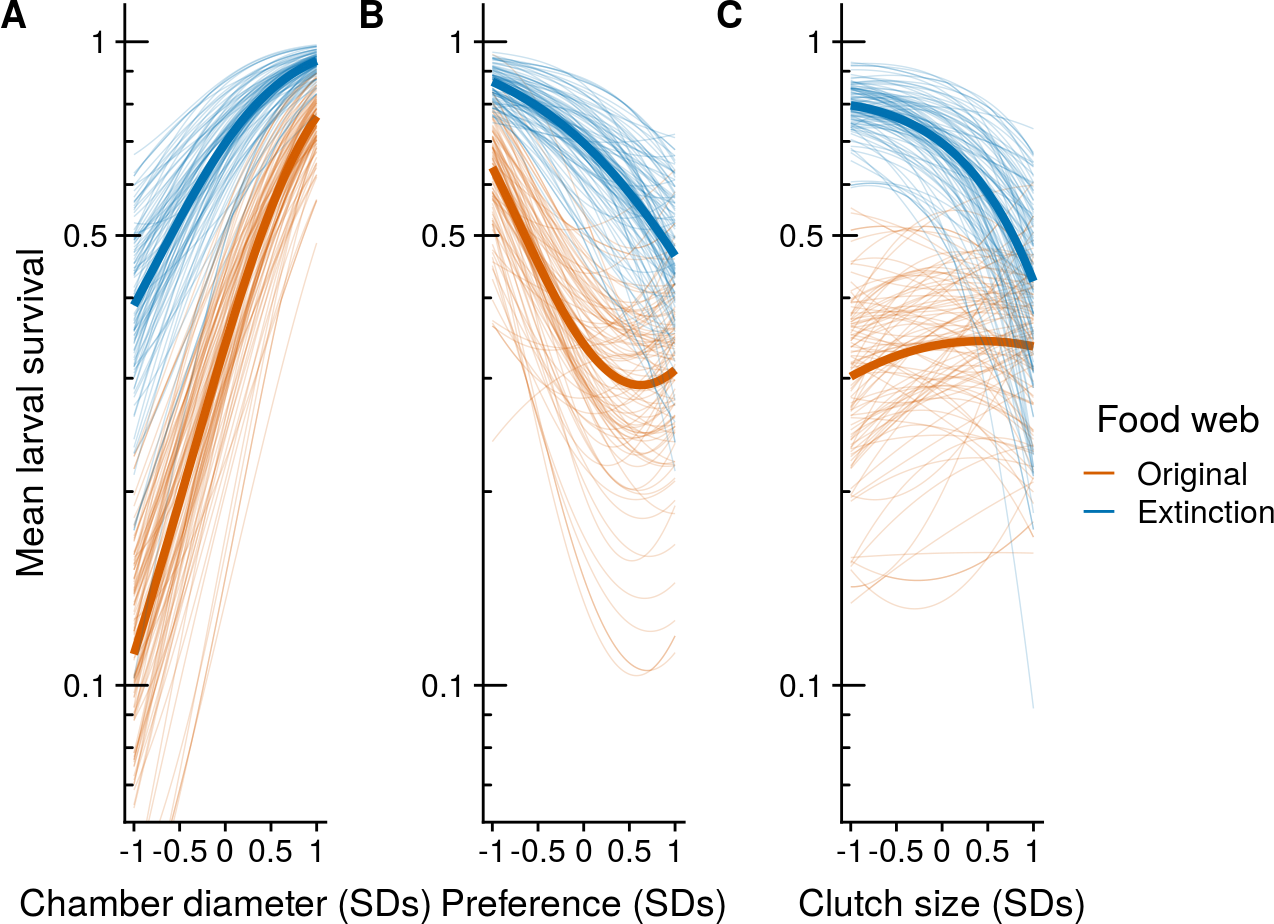
\includegraphics{Univariate-Fitness-Landscapes-1.png}
\caption{Selection gradients acting on \texit{Iteomyia} traits in complex vs. simple food webs. Each panel corresponds to a different phenotypic trait: chamber diameter (A); clutch size (B); and female preference (C). Solid lines represent the estimated gradients in complex (orange) and simple (blue) food webs. Transparent lines represent bootstrapped replicates (n=100) to show the uncertainty in estimated gradients. Note that only 100 bootstraps are displayed here, but that inferences are based on 1,000 bootstrapped samples.}
\label{Fig:FL_1D}
\end{figure}

\begin{figure}[h!]
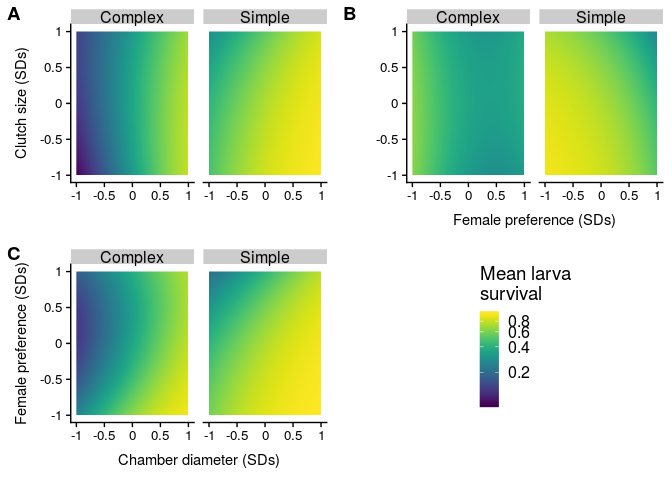
\includegraphics{Multivariate-Fitness-Landscapes-1.png}
\caption{Fitness landscapes of gall traits in complex vs. simple food webs. Each panel corresponds to a different combination of traits: clutch size and chamber diameter (A); clutch size and female preference (B); female preference and chamber diameter (C). Note that traits for all plots range 1 SD below and above the mean (=0).}
\label{Fig:FL_2D}
\end{figure}

%%%%%%%%%%%%%%%%%%%%%
% Videos
%%%%%%%%%%%%%%%%%%%%%
% If you have videos, journal style for them is similar to that for
% figures. You'll want to include a still image (such as a JPEG)
% to give your readers a preview of what the video looks like.

%%%%% Include the text below if you have videos

\renewcommand{\figurename}{Video} 
\setcounter{figure}{0}
% Thanks to Flo Debarre for the pro tip of putting
% \renewcommand{\figurename}{Video} before the Video legend and
% \renewcommand{\figurename}{Figure} after it!

\begin{figure}[h!]
%\includegraphics{VideoScreengrab.jpg}
\caption{Video legends can follow the same principles as figure legends. Counters should be set and reset so that videos and figures are enumerated separately.}
\label{VideoExample}
\end{figure}

\renewcommand{\figurename}{Figure}
\setcounter{figure}{1}

%%%%% Include the above if you have videos


\begin{figure}[h!]
%\includegraphics{elegance}
\caption{In this way, figure legends can be listed at the end of the document, with references that work, even though the graphic itself should be included for final files after acceptance. Instead, upload the relevant figure files separately to Editorial Manager; Editorial Manager should insert them at the end of the PDF automatically.}
\label{Fig:AnotherFigure}
\end{figure}

\subsection*{Online figure legends}

\renewcommand{\thefigure}{A\arabic{figure}}
\setcounter{figure}{0}

\begin{figure}[h!]
%\includegraphics{jumps20m}
\caption{\textit{A}, the quick red fox proceeding to jump 20~m straight into the air over not one, but several lazy dogs. \textit{B}, the quick red fox landing gracefully despite the skepticism of naysayers.}
\label{Fig:Jumps}
\end{figure}

\begin{figure}[h!]
%\includegraphics{jumps20m}
\caption{The quicker the red fox jumps, the likelier it is to land near an okapi. For further details, see \citet{LemKapEx07}.}
\label{Fig:JumpsOk}
\end{figure}

\renewcommand{\thefigure}{B\arabic{figure}}
\setcounter{figure}{0}

\end{document}
